% !Mode:: "TeX:UTF-8" (encoding info for WinEdt)
\section{Elexis-Bildanzeige}
Einbinden von Fotos und anderen Bildern in den Konsultationstext. Dieses Plugin ist Teil der Standard-Distribution. Um ein externes Bild einzubinden, gehe Sie so vor:
 Bewegen Sie den Cursor an die Stelle, wo das Bild eingefügt werden soll, und klicken Sie mit der rechten Maustaste

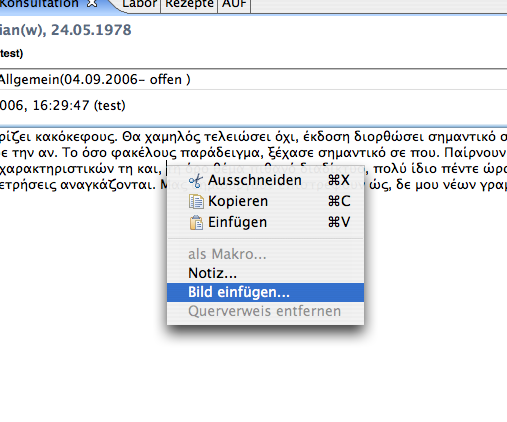
\includegraphics[width=4in]{images/bild1}
% bild1.png: 507x422 pixel, 72dpi, 17.89x14.89 cm, bb=0 0 507 422


Klicken Sie \textit{Bild einfügen...} und wählen Sie in der darauf öffnenden Dateiauswahlbox das gewünschte Bild aus (Es sollte im JPG, GIF oder PNG-Format sein). Das Bild wird in die Datenbank importiert und eine Referenz darauf wird im Text eingefügt (Das Originalbild wird danach nicht mehr benötigt).

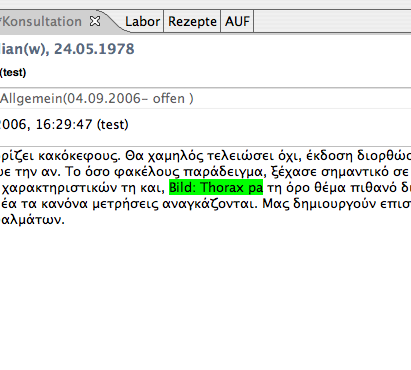
\includegraphics[width=3in]{images/bild2}
% bild2.png: 411x370 pixel, 72dpi, 14.50x13.05 cm, bb=0 0 411 370


Mit einem Klick auf diesen Querverweis kann das Bild jederzeit wieder angezeigt werden.

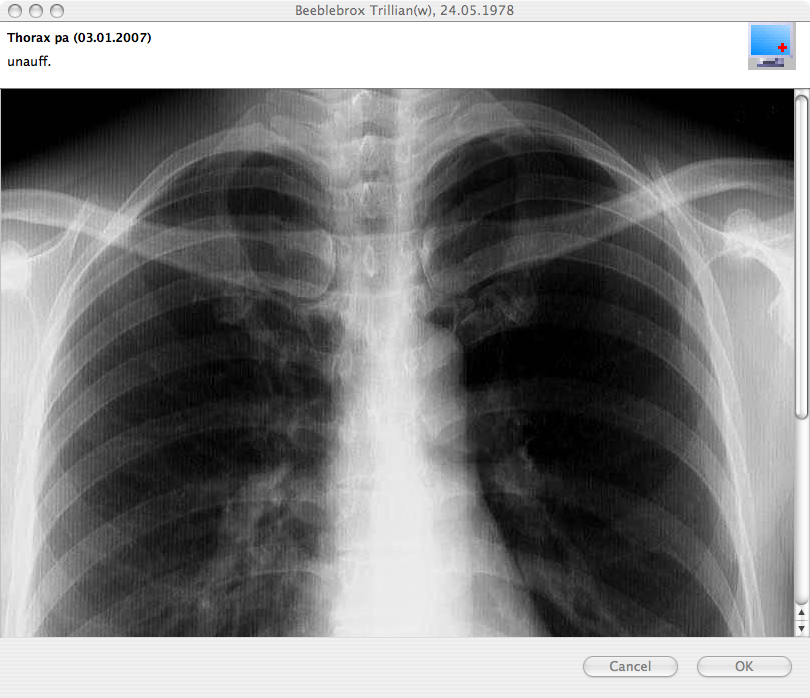
\includegraphics[width=4in]{images/bild3}
% bild3.png: 810x698 pixel, 72dpi, 28.58x24.62 cm, bb=0 0 810 698
